\section{Landscape geometry}

\label{2305:app:landscape}
In this appendix we discuss the landscape of the population risk for the phase retrieval problem $p=1$. We start by discussing the Euclidean case first, moving to the sphere next. 

We recall the reader that the loss function is given by given by:
\begin{align}
\label{2305:eq:app:poprisk}
\ell(w) \coloneqq \ell(y,f_{\Theta}(x)) =  \frac{1}{2}\left((w_{\star}^{\top}x)^2+\sqrt{\Delta}z-(w^{\top}x)^2\right)^2
\end{align}
As before, we define the pre-activations (or local fields):
\begin{align}
    \lambda_{\star} = w_{\star}^{\top}x, && \lambda = w^{\top}x
\end{align}
and the displacement vector:
\begin{align}
    \mathcal{E}(w) &\coloneqq (w_{\star}^{\top}x)^2+\sqrt{\Delta}z-(w^{\top}x)^2 \notag\\
    &=  \lambda_{\star}^2 + \sqrt{\Delta}z-\lambda^2
\end{align}
Note that:
\begin{align}
    \nabla_{w}\mathcal{E}(w) = -2\lambda x
\end{align}
Therefore, the Euclidean gradient of the loss is given by:
\begin{align}
    \nabla_w \ell(w) =-2 \mathcal{E}(w)\lambda x
\end{align}
And the Euclidean Hessian is:
\begin{align}
    \nabla^2 \ell(w) &= 2\left(2\lambda^2-\mathcal{E}(w)\right) xx^{\top} \notag\\
    &=2(3\lambda^2-\lambda_{\star}^2+\sqrt{\Delta}z)xx^{\top}
\end{align}
% \begin{align}
% \label{2305:eq:app:poprisk}
% \mathcal{R}(w) \coloneqq  \frac{1}{2}\mathbb{E}\left[\left((w_{\star}^{\top}x)^2-(w^{\top}x)\right)^2\right]+\frac{\Delta}{2}, && x\sim\mathcal{N}(0,\sfrac{1}{d}I_{d})
% \end{align}
\paragraph{Averaged geometry ---} We now compute the expected geometry by taking population averages of the above. It will be useful to define the correlation variables:
\begin{align}
   \rho = \frac{||w_{\star}||^2}{d}, && m = \frac{w_{\star}^{\top}w}{d}, && q = \frac{||w||^2}{d}
\end{align}
 which we recall are the second moments of the pre-activations $(\lambda_{\star},\lambda)$. With this notation, the population risk (the expected value of \eqref{2305:eq:app:poprisk}) reads:
\begin{align}
    \mathcal{R}(m,q) =\sfrac{\Delta}{2}+ \frac{3}{2}\rho^2+\frac{3}{2}q^2-2m^2-\rho q
\end{align}
In order to compute the expected gradient, we need the following moments (for readability we omit throughout the overall factor \(\sfrac1d\) coming from the covariance \(\Sigma=\sfrac1d I\), which rescales the gradient and Hessian but changes neither the critical points nor the signs of the Hessian eigenvalues):
\begin{align}
    \mathbb{E}[\lambda_{\star}^2\lambda x] = \rho w+2m w_{\star}, && \mathbb{E}[\lambda^3 x] = 3q w
\end{align}
Which gives:
\begin{align}
    \nabla_{w}\mathcal{R}(w) = -2\mathbb{E}\left[\mathcal{E}(w)\lambda x\right]= -2((\rho-3q) w+2m w_{\star})
\end{align}
Finally, let's compute the expected Hessian. For that, we will need the following moments:
    \begin{align}
        \mathbb{E}[\lambda^{2}_{\star}xx^{\top}] = \rho I_{d}+w_{\star}w_{\star}^{\top}, && \mathbb{E}[\lambda^{2}xx^{\top}] = q I_{d}+w w^{\top}
    \end{align}
    Therefore:
    \begin{align}
        \nabla_{w}^2\mathcal{R}(w) = 2\mathbb{E}\left[(3\lambda^2-\lambda_{\star}^2+\sqrt{\Delta}z)xx^{\top}\right]=2\left(-(\rho-3q)I_{d}+3w w^{\top}-w_{\star}w_{\star}^{\top}\right)
    \end{align}
    We are now ready to compute the critical points of the Euclidean landscape and evaluate their nature. By definition, the critical points are defined as solutions of $\nabla_{w}\mathcal{R}(w)=0$. These are:
\begin{itemize}
    \item $w = 0$ ($(m,q) = (0,0)$): The Hessian of this critical point is given by:
    \begin{align}
        \nabla_{w}^{2}\mathcal{R}(0) = -2(\rho I_{d}+w_{\star}w_{\star}^{\top}) \prec 0
    \end{align}
    This is a negative-definite matrix with $d-1$ negative eigenvalues $-2\rho$ and one negative eigenvalue $-2(\rho+1)$ with eigenvector $w_{\star}$. Therefore, this is a local maximum. The risk associated is given by: 
    \begin{align}
        \mathcal{R}(0) = \frac{\Delta}{2}+\frac{3}{2}\rho^2
    \end{align}
    \item $(m,q) = (0,\sfrac{\rho}{3})$: This defines a line of critical points $\{w \in\mathbb{R}^{d}: w \perp w_{\star} \text{ and }||w|| = \sfrac{1}{\sqrt{3}}||w_{\star}||\}$. The Hessian is given by:
    \begin{align}
        \nabla_{w}^{2}\mathcal{R} = 2(3ww^{\top}-w_{\star}w_{\star}^{\top}) 
    \end{align}
    Note this is a rank-two matrix with $d-2$ zero eigenvalues (associated to flat directions), one negative eigenvalue with eigenvector $w_{\star}$ and a positive eigenvalue with eigenvector perpendicular to the minima. This is a saddle-point, and have population risk:
    \begin{align}
        \mathcal{R}(0,\sfrac{\rho}{3}) = \frac{\Delta}{2}+\frac{4}{3}\rho^2
    \end{align}
    \item $w=\pm w_{\star}$ ($(m,q) = (\pm\rho,\rho)$): From the definition of our problem, this is the global minima. The expected Hessian is given by:  
    \begin{align}
        \nabla_{w}^{2}\mathcal{R}(\pm w_{\star}) = 4(\rho I_{d}+w_{\star}w_{\star}^{\top}) \succ 0
    \end{align}
    which is indeed a positive definite matrix. This defines the minimum achievable population risk:
    \begin{align}
        \underset{w\in\mathbb{R}^{d}}{\min}~\mathcal{R}(w) = \mathcal{R}(\pm\rho,\rho) = \frac{\Delta}{2}
    \end{align}
\end{itemize}
This is consistent with the discussion in \cite{chen2019gradient}, where the critical points and their nature were reported, but explicit expressions for the expected gradient and Hessian were not given. 
From this geometry, a neat picture for the one-pass SGD dynamics in the unconstrained problem can be drawn. Consider $w_{\star}\in\mathbb{S}^{d-1}$ with a random initialization at high-dimensions:
\begin{align}
    w^{0}\sim\mathcal{N}(0,I_{d}).
\end{align}
Note that with high-probability the random initial weights is almost orthogonal to the signal, and we have $(m,q)\approx (0,1)$. Note this is not a critical point, and the initial gradient $\nabla_{w}\mathcal{R}(w^{0}) = 4 w^{0}$ is orthogonal to $w_{\star}$. Indeed, for $p=1$ and $\Delta=0$ the unconstrained ODEs \eqref{2305:eq:overlapping_ODE} are given by:
\begin{align}
\label{2305:eq:app:odes:highd}
\dot{m}(t) &= 6 ~m(t) (\rho-q(t))\\
\dot{q}(t) &= 4\left(q(t)(\rho-3q(t))+2m(t)^2\right) \notag\\
&\quad + 12\gamma\left(q(t)(\rho^2 + 5q(t)^2-2\rho q(t))+4m^2(\rho-2q(t))\right)
\end{align}
 where $\dot{} \coloneqq \sfrac{\dd}{\dd t}$ and we dropped the bars for clarity. Therefore, in the initial stage of the dynamics $\dot{m}\approx 0$ remains almost constant, while $q$ decreases, and the dynamics flow in the direction of the saddle-point $(0,\sfrac{\rho}{3})$. As we have seen, the saddle is mostly flat, with a single negative curvature direction pointing towards $w_{\star}$. This is precisely the mediocrity stage, where the dynamics slows down and SGD gets stuck for a long time before being able to develop significant correlation with $w_{\star}$ and escape.

\subsection{Landscape in the sphere}
\label{2305:sec:app:spherical}
Recall that the orthogonal projector on a vector $u\in\mathbb{S}^{d-1}$ is given by:
\begin{align}
    {\rm Proj}_{u}  = I_{d} - uu^{\top}
\end{align}
Therefore, the gradient on the sphere is given by:
\begin{align}
    {\rm grad}_{\mathbb{S}^{d-1}}\ell(w) &= {\rm Proj}_{\mathbb{S}^{d-1}}(\nabla_{w}\ell(w)) = (I_{d}-ww^{\top})\nabla_{w}\ell(w) \notag\\
    &=-2\mathcal{E}(w)\lambda (x-\lambda w)
\end{align}
Similarly, the Hessian on the sphere can be written as:
\begin{align}
    {\rm Hess}_{\mathcal{S}^{d-1}}\ell(w) &= {\rm Proj}_{\mathbb{S}^{d-1}}\left(\nabla_{w}^{2}\ell(w)\right)-\langle w, \nabla_{w}\ell(w)\rangle I_{d}\notag\\
    &=(3\lambda^2-\lambda_{\star}^{2})(xx^{\top}-\lambda w x^{\top})+\mathcal{E}(w)\lambda^2 I_{d}
\end{align}
\begin{figure}
    \centering
    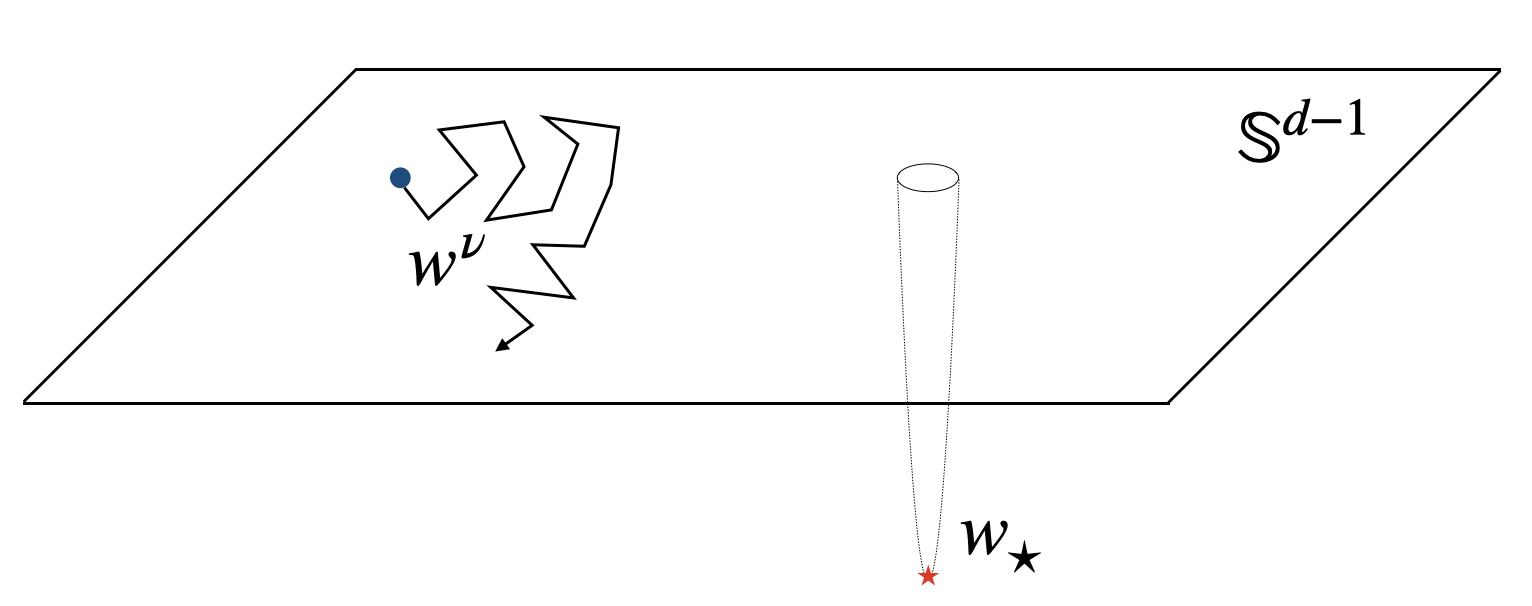
\includegraphics[width=0.8\textwidth]{figs/landscape}
    \caption{Low-dimensional illustration of mediocrity at initialization. As discussed in Section~\ref{2305:sec:app:spherical}, the expected Hessian at initialization is a strict saddle-point with $d-1$ flat directions and a single negative direction pointing towards the global minimum. This scenario is particularly hard for descent based algorithms such as SGD, that require $n=d\log{d}$ samples / steps to develop significant correlation with the signal.}
    \label{2305:fig:app:landscape}
\end{figure}
\paragraph{Averaged geometry ---} Recall that in the sphere we have $\rho=q=1$. Therefore, the population risk now only depends on the correlation $m=\langle w_{\star}, w\rangle$, and reads:
\begin{align}
    \mathcal{R}(w) = 2(1-m^2)+\frac{\Delta}{2}
\end{align}
Luckily, half of the moments we need have been already computed above. To get the gradient on the sphere, we just need to compute: 
\begin{align}
    \mathbb{E}[\lambda_{\star}^2\lambda^2] = 1+2m^2, && \mathbb{E}[\lambda^4] = 3
\end{align}
Therefore, the averaged spherical gradient is given by:
\begin{align}
   {\rm grad}_{\mathbb{S}^{d-1}}\mathcal{R}(w) = 4m\left(m w-w_{\star}\right)
\end{align}
We also have all moments required to compute the expected spherical Hessian:
\begin{align}
 {\rm Hess}_{\mathcal{S}^{d-1}}\mathcal{R}(w) = 4\left[m^2 I_{d}+m w w_{\star}^{\top}-w_{\star}w_{\star}^{\top}\right]
\end{align}
As before, we can now analyze the critical points and their nature.
\begin{itemize}
    \item $w\perp w_{\star}$ ($m=0$): The Hessian is given by: 
    \begin{align}
        {\rm Hess}_{\mathcal{S}^{d-1}}\mathcal{R}(w) = -4w_{\star}w_{\star}^{\top}
    \end{align}
    Which is a rank one matrix with $d-1$ eigenvalues $0$ (flat directions) and a single negative eigenvalue $-4$ with negative curvature pointing towards the signal $w_{\star}$. Therefore, this is a strict saddle-point. However, since the risk is a decreasing function of $m^2 \in [0,1]$, this is also the global maximum of the risk.
    
    \item $w=\pm w_{\star}$ ($m=\pm 1$): As before, these are the global minima, and define the minimal achievable risk $\mathcal{R}(\pm w_{\star}) = \sfrac{\Delta}{2}$. Indeed, the Hessian is given by:
    \begin{align}
        {\rm Hess}_{\mathcal{S}^{d-1}}\mathcal{R}(\pm w_{\star}) = 4 I_{d}\succ 0
    \end{align}
   which is positive-define.
\end{itemize}
Therefore, the landscape now resembles a golf course: completely flat with a single whole corresponding with the global minimum $w_{\star}$, see Figure~\ref{2305:fig:app:landscape} for an illustration. This is the prototypical image of mediocrity. In particular, differently from the unconstrained case, random initialization
\begin{align}
    w^{0}\sim {\rm Unif}(\mathbb{S}^{d-1}(\sqrt{d})) 
\end{align}
now corresponds to initializing close to the saddle-point point $m^{0}=0$: with high-probability the initial weights are orthogonal to the signal at high-dimensions: 
\begin{align}
    m^{0}=\sfrac{1}{d}\langle w^{0},w_{\star}\rangle\approx  \sfrac{1}{\sqrt{d}}\ll 1.
\end{align} 
For the reader convenience, we recall that the ODEs \eqref{2305:eq:spherical-p1-ode} describing the evolution of the correlation $m$ is given by:
\begin{align}
  \dot{m}(t) &= m{(t)}\left[4(1-6\gamma)(1-m^2{(t)})-2\gamma\Delta\right]
\end{align}
Close to initialization we now have $\dot{m}(0) \approx 0$, slowing down the dynamics close to initialization.
%%%%%%%%%%%%%%%%%%%%%%%%%%%%%%%%%%%%%%%%%%%%%%%%%%%%%%%%%%%%%%%%%%%%%%%%%%%%%%%
